\subsection*{\textcolor{subsectioncolor}{\textsf{4. \textit{TEST PROCEDURES}}}}
\addcontentsline{toc}{subsection}{4. \textit{TEST PROCEDURES}}


\subsubsection*{\textit{Server}}

Pengujian subsistem ini dilakukan dengan menggunakan subsistem \textit{server} yang sudah mencakup modul ServerSocket dan DialogueManager,
dan dibantu dengan program pengujian modul ClientSocket,
yang berperan sebagai \textit{client} sederhana berbentuk konsol dengan masukan dan keluaran teks.
Gambar \ref{ServerOnServerTest} dan Gambar \ref{ClientOnServerTest} menunjukkan proses pengujian subsistem ini.

\begin{figure}
\centering
\subfloat[\textit{Server}]{\label{ServerOnServerTest}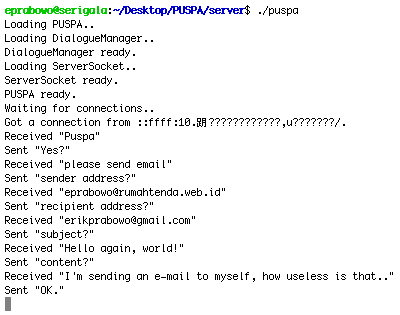
\includegraphics[width=0.5\textwidth]{ServerOnServerTest}}
\subfloat[\textit{Client}]{\label{ClientOnServerTest}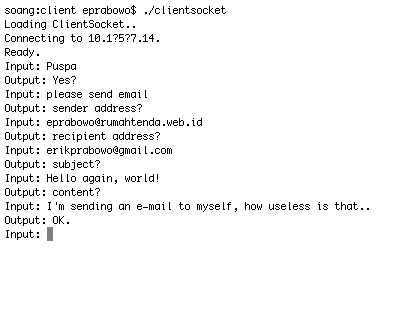
\includegraphics[width=0.5\textwidth]{ClientOnServerTest}}
\caption{Pengujian subsistem \textit{server}}
\label{ServerTest}
\end{figure}


\subsubsection*{\textit{Client}}

Pengujian subsistem ini dilakukan dengan menggunakan subsistem \textit{client} yang sudah mencakup modul ClientSocket, Synthespian, dan UserInterface,
dan dibantu dengan program pengujian modul ServerSocket,
yang berperan sebagai \textit{server} sederhana yang hanya mengembalikan karakter-karakter yang sama dengan masukan yang didapat dari subsistem \textit{client}.
Gambar \ref{ClientOnClientTest} dan Gambar \ref{ServerOnClientTest} menunjukkan proses pengujian subsistem ini.

\begin{figure}
\centering
\subfloat[\textit{Kalimat 1}]{\label{ClientOnClientTest1}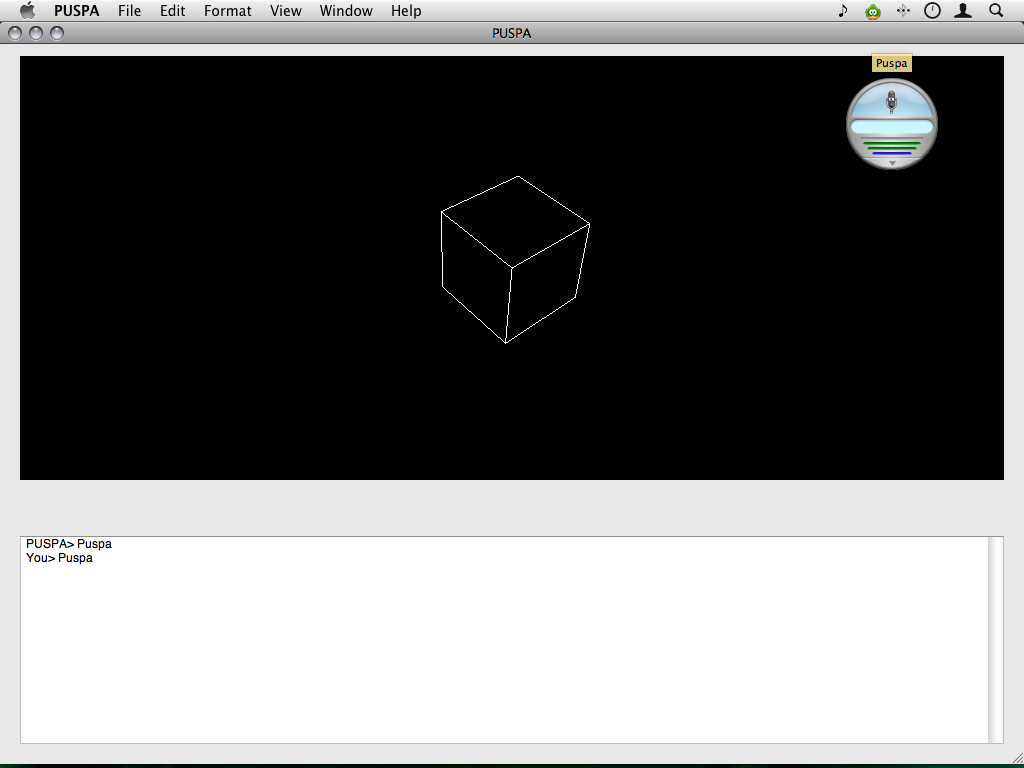
\includegraphics[width=0.5\textwidth]{ClientOnClientTest1}}
\subfloat[\textit{Kalimat 2}]{\label{ClientOnClientTest2}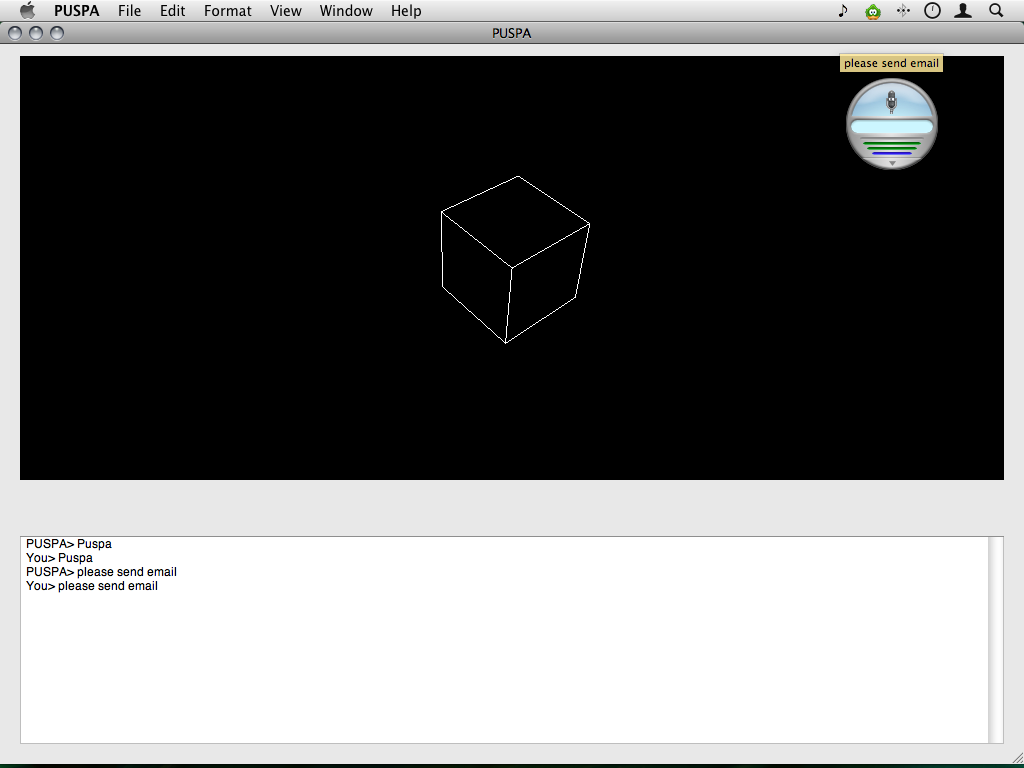
\includegraphics[width=0.5\textwidth]{ClientOnClientTest2}}\\
\subfloat[\textit{Kalimat 3}]{\label{ClientOnClientTest3}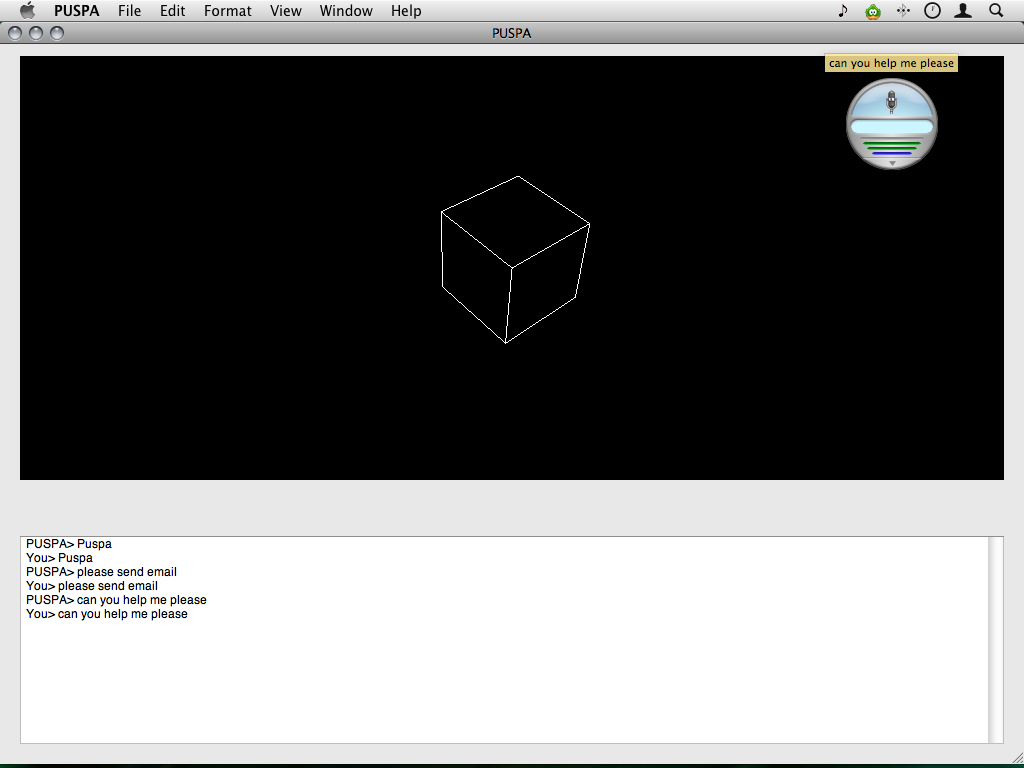
\includegraphics[width=0.5\textwidth]{ClientOnClientTest3}}
\subfloat[\textit{Kalimat 4}]{\label{ClientOnClientTest4}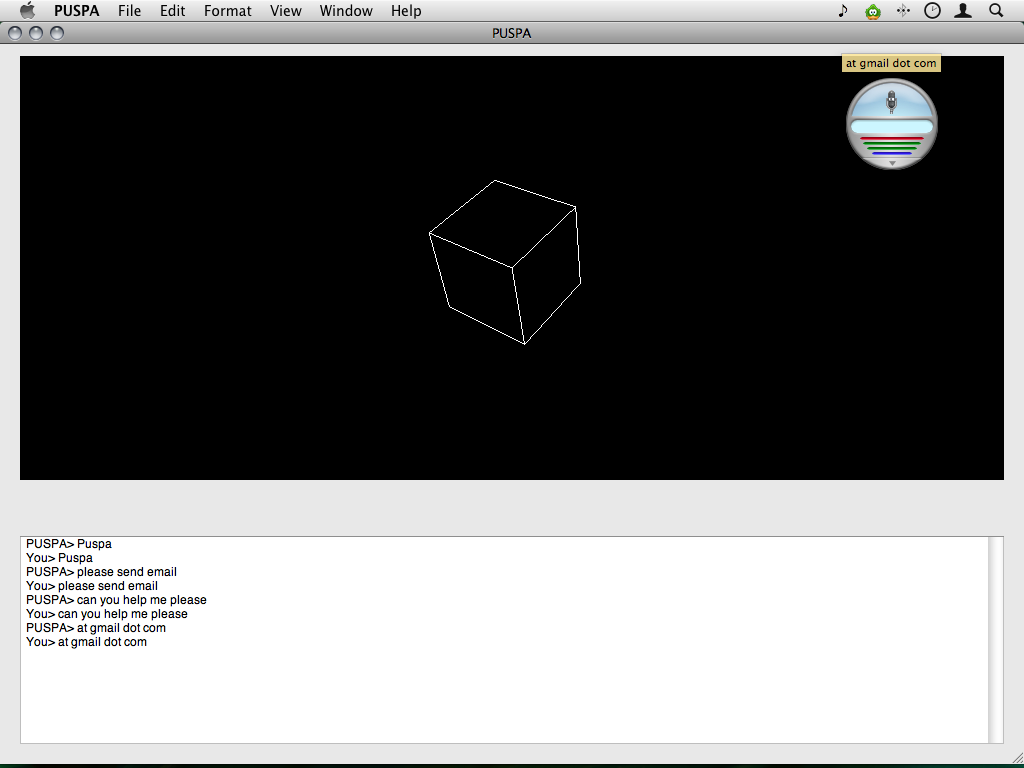
\includegraphics[width=0.5\textwidth]{ClientOnClientTest4}}
\caption{Pengujian subsistem \textit{client}}
\label{ClientOnClientTest}
\end{figure}

\begin{figure}
\centering
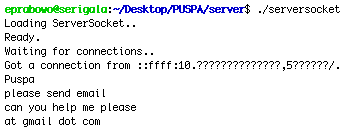
\includegraphics[width=0.5\textwidth]{ServerOnClientTest}
\caption{Yang terjadi pada \textit{server} (sederhana) saat subsistem \textit{client} diuji}
\label{ServerOnClientTest}
\end{figure}
